\chapter{Theoretical Framework \label{cap:teo}}

In this chapter, the analytical-theoretical tools that allow for the description of the photonic systems studied in this thesis will be developed. These systems consist of the propagation of low-power laser light\footnote{1 mW output power, within the safety regime of Class 3b lasers.} propagated in coupled systems of waveguides, which are written inside a borosilicate wafer. These experimental conditions allow the behavior of light to be described using Maxwell's equations applied to a linear, isotropic, non-magnetic medium without free charge or current sources.
\section{Light Propagation in Dielectric Waveguides from Maxwell's Equations \label{cap:maxwell}}

The Maxwell's equations in this regime, in the International System of Units (SI), are:
\begin{align}
	\nabla\cdot\left[\varepsilon(\textbf{r})\textbf{E}\right] &= 0 \ , \label{eqn:gauss}
	\\	
	\nabla\times\textbf{E} &= -\mu_0 \frac{\partial \textbf{H}}{\partial t} \ , \label{eqn:faraday-lenz}
	\\	
	\nabla\cdot\textbf{H} &= 0 \ , \label{eqn:div0}
	\\	
	\nabla\times\textbf{H} &=\varepsilon(\textbf{r}) \frac{\partial \textbf{E}}{\partial t} \ , \label{eqn:ampere-maxwell}
\end{align}

where \textbf{E} is the electric field and \textbf{H} is the magnetic field. In general, the waveguides considered are systems that are invariant in the direction of propagation $\hat{\textbf{z}}$. Therefore, the refractive index profile can be expressed as $n(x,y) = n_0 + \Delta n(x,y)$, where $n_0 = 1.48$ is the refractive index of the borosilicate substrate and $\Delta n(x,y)$ represents the transverse modulation of the index, with maximum values in the range of $10^{-5} - 10^{-3}$. This spatial variation of the index, $\Delta n(x,y)$, is responsible for the optical confinement in the transverse plane $(x,y)$, allowing for the guided propagation of electromagnetic modes along the $\hat{\textbf{z}}$ axis.

After assuming a harmonic time dependence proportional to $e^{-i\omega t}$ Faraday-Lenz's law (\ref{eqn:faraday-lenz}) can be substituted into Ampère-Maxwell's law (\ref{eqn:ampere-maxwell}), yielding:
\begin{align}
	\nabla\times\left(\frac{\nabla\times\textbf{E}}{i\omega\mu_0}\right) &= -i\omega \varepsilon_0 n^2 \textbf{E} \implies \nabla\times\nabla\times\textbf{E} = k_0^2n^2\textbf{E} \ , \label{eqn:rotordoble}
\end{align}
where $k_0 \equiv \omega/c$ is the vacuum wavenumber. By vector calculus identity, it holds that: $\nabla\times\nabla\times\textbf{E} = \nabla(\nabla\cdot\textbf{E}) - \nabla^2\textbf{E}$. Gauss' law implies that (\ref{eqn:gauss}) implica que $\nabla\cdot \textbf{E} = -\frac{\nabla n^2}{n^2}\cdot\textbf{E}$. Substituting into equation (\ref{eqn:rotordoble}), we obtain the following:
\begin{equation}
	\left(\nabla^2  + k_0^2n^2\right)\textbf{E} = -\nabla\left( \frac{\nabla n^2}{n^2} \cdot \textbf{E}  \right) \ . \label{eqn:helmholz}
\end{equation}
Similarly, it is possible to combine Ampère-Maxwell's (\ref{eqn:ampere-maxwell}) and Faraday-Lenz's (\ref{eqn:faraday-lenz}) equations together with the null divergence of the magnetic field \textbf{H} (\ref{eqn:div0}):
\begin{align}
	\nabla\times \left(\frac{\nabla\times\textbf{H}}{-i\omega \varepsilon_0 n^2}\right) = i\omega \mu_0 \textbf{H} &\implies \nabla\times \left(\frac{1}{n^2}\nabla\times\textbf{H}\right) = k_0^2 \textbf{H} \ ,
	\nonumber
	\\
	\nabla\times\nabla\times\textbf{H} + \nabla n^2 \times \left( \nabla\times\textbf{H}\right)
	&= 
	  k_0^2 n^2\textbf{H} \ .
	 	\nonumber
\end{align}
The analogous equation to (\ref{eqn:helmholz}) for \textbf{H} is therefore:
\begin{align}
	 \left(\nabla^2  + k_0^2 n^2 \right) \textbf{H} &= i\omega \epsilon_0 \nabla n^2 \times \textbf{E} \ .
	 \label{eqn:helmholzH}
\end{align}
In this thesis, we will work with systems in which light travels through a waveguide structure that is invariant in the $\hat{\mathbf{z}}$ direction and periodic in the transverse direction. It is therefore useful to separate the longitudinal and transverse components of the fields, assuming a plane-wave dependence of the form $e^{i k_z z}$ in the spatial variable $z$:
\begin{align}
	\nabla_\perp \times  \textbf{E} + ik_z \hat{\textbf{z}} \times \textbf{E} &= i\omega\mu_0\textbf{H} \ ,
	\label{eqn:EfieldH}
	\\
	\nabla_\perp \times  \textbf{H} + ik_z \hat{\textbf{z}} \times \textbf{H} &= -i\omega \epsilon_0 n^2 \textbf{E} \ .
	\label{eqn:HfieldE}
\end{align}
If we consider the decompositions $\textbf{E}=\textbf{E}_\perp +\hat{\textbf{z}} E_z$ and $\textbf{H}=\textbf{H}_\perp +\hat{\textbf{z}} H_z$, $\nabla_\perp \equiv - \hat{\textbf{z}}\times (\hat{\textbf{z}}\times\nabla)   $, the Maxwell's equations involving curls can be written as:
\begin{align}
	\nabla_\perp \times  \textbf{E}_\perp + ik_z \hat{\textbf{z}} \times \textbf{E}_\perp + \nabla_\perp \times (\hat{\textbf{z}} E_z) &= i\omega\mu_0(\textbf{H}_\perp +\hat{\textbf{z}} H_z) \ ,
	\label{eqn:Efield}
	\\
	\nabla_\perp \times  \textbf{H}_\perp + ik_z \hat{\textbf{z}} \times \textbf{H}_\perp + \nabla_\perp \times (\hat{\textbf{z}} H_z) &= -i\omega \epsilon_0 n^2 (\textbf{E}_\perp +\hat{\textbf{z}} E_z) \ .
	\label{eqn:Hfield}
\end{align}
After applying the cross product in the $\hat{\textbf{z}}$ direction to equations (\ref{eqn:Efield}) and (\ref{eqn:Hfield}),  $E_z$ y $H_z$  can be expressed in terms of $\textbf{E}_\perp$ and $\textbf{H}_\perp$:
\begin{equation*}
\begin{aligned}[c]
	 -i\nabla_\perp E_z &= k_z\textbf{E}_\perp +\omega \mu_0 \hat{\textbf{z}} \times \textbf{H}_\perp \ ,
	 	  	 \\
	 	  	i\hat{\textbf{z}} \times \nabla_\perp H_z &= k_z \hat{\textbf{z}} \times\textbf{H}_\perp + \omega\epsilon_0 n^2 \textbf{E}_\perp \ ,
\end{aligned} 
\quad
\begin{aligned}[c]
	-i \nabla_\perp H_z &= k_z \textbf{H}_\perp - \omega \epsilon_0 n^2  \hat{\textbf{z}} \times \textbf{E}_\perp \ ,
	\\
	i\hat{\textbf{z}} \times\nabla_\perp E_z &=  \omega \mu_0 \textbf{H}_\perp+k_z  \hat{\textbf{z}} \times \textbf{E}_\perp \ .
\end{aligned}
\end{equation*}
Finally, the perpendicular components of the fields,  $\textbf{H}_\perp$ y $\textbf{E}_\perp$, can be expressed in terms of the longitudinal components, $H_z$ y $E_z$:
\begin{equation}
\begin{aligned}[c]
 \hat{\textbf{z}} \times \textbf{H}_\perp &= i\frac{(\omega\epsilon_0 n^2 \nabla_\perp E_z  - \hat{\textbf{z}} \times \nabla_\perp H_z k_z)}{k_0^2 n^2 - k_z^2} \ ,
 \\
\textbf{H}_\perp &= \frac{i}{k_0^2 n^2 - k_z^2}\left(k_z\nabla_\perp H_z + \omega \epsilon_0 n^2\hat{\textbf{z}} \times \nabla_\perp E_z\right) \ ,
\end{aligned}
\begin{aligned}[c]
	\hat{\textbf{z}} \times \textbf{E}_\perp &= -i\frac{(k_z\hat{\textbf{z}} \times \nabla_\perp E_z + \omega\mu_0 \nabla_\perp H_z)  }{k_0^2 n^2 - k_z^2} \ ,
	\\
\textbf{E}_\perp &= \frac{i}{k_0^2 n^2 - k_z^2}\left(k_z \nabla_\perp E_z - \omega\mu_0 \hat{\textbf{z}} \times \nabla_\perp H_z\right) \ . \label{eqn:transversal}
\end{aligned}
\end{equation}
Equations (\ref{eqn:helmholz}), (\ref{eqn:helmholzH}), and (\ref{eqn:transversal}) will serve as the analytical tools for the two case studies in the following sections.
\section{Analytical solutions for one-dimensional slab-type waveguides \label{cap:slab}}
The simplest system that can be studied is a slab waveguide, whose analytical form for the refractive index $n(x)$ is as follows:
\begin{equation*}
	n(x) = \left\{\begin{matrix}
	n_1 \ , \quad |x| \le a
	\\
	n_0 \ , \quad |x| > a
 	\end{matrix}\right. \ ,
\end{equation*}
with $n_1 > n_0$. \begin{figure}[H]
	\centering
	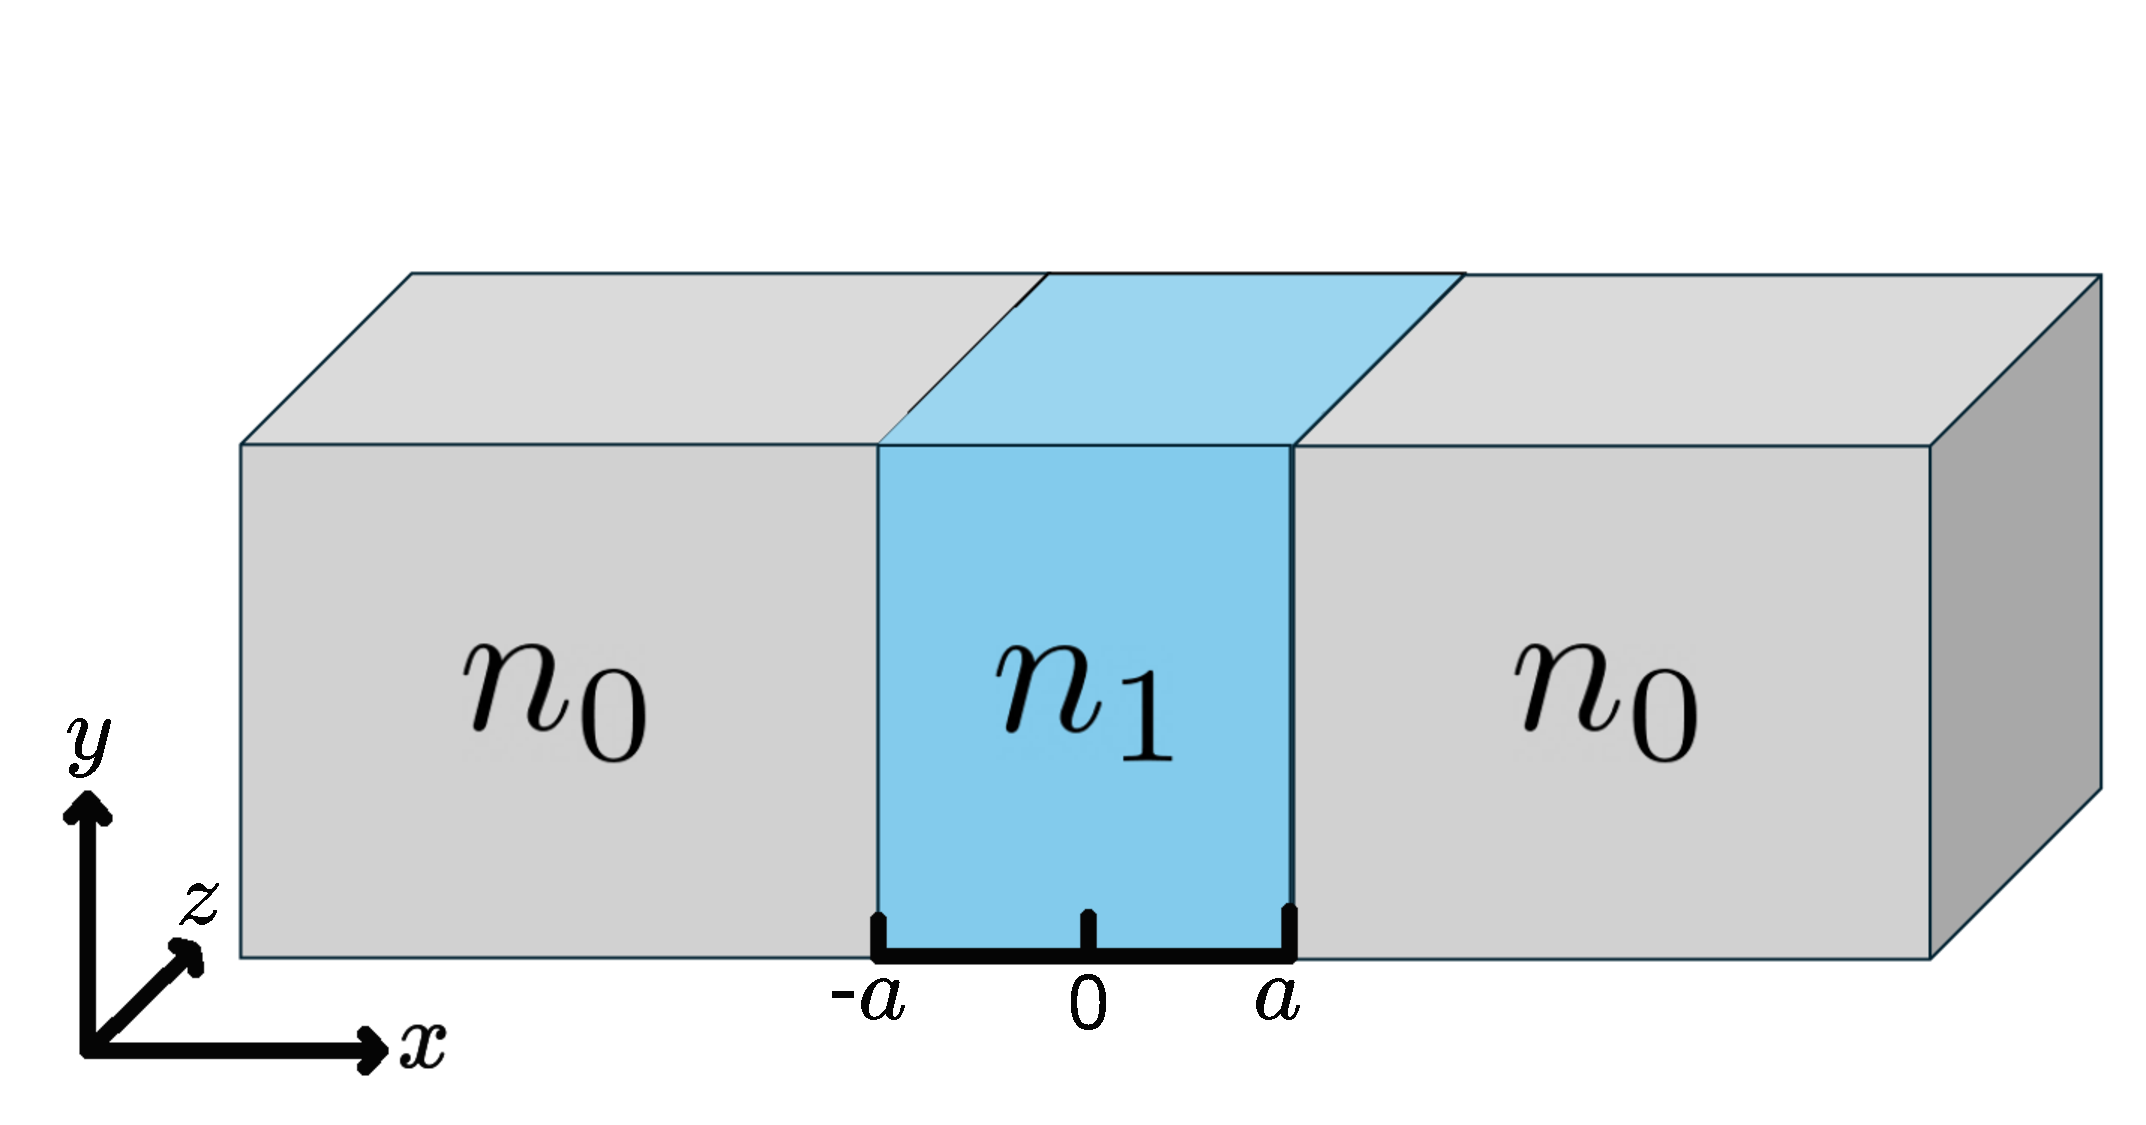
\includegraphics[width=0.6\linewidth]{media/slab.pdf}
	\caption[Shape of a slab-type waveguide.]{Shape of a slab-type waveguide. The structure is invariant in the $\mathbf{\hat{y}}$ (vertical) and $\mathbf{\hat{z}}$ (into the page) directions.}
\end{figure} Since $\nabla n^2 = \textbf{0}$ para $|x| \neq a$, the right-hand sides of equations (\ref{eqn:helmholz}) and (\ref{eqn:helmholzH}) are of the Helmholtz type. Defining $\Psi = \{E_z, H_z\} $:
\begin{align*}
	(\nabla_\perp^2  + k_0^2n^2 - k_z^2) \Psi  &=  \frac{d^2\Psi}{dx^2} + (k_0^2n^2 - k_z^2) \Psi  = 0 \ .
\end{align*}
Since $n(x)=n(-x)$, the solutions $\Psi$ must be even or odd. Indeed, if  $\Psi(x)$ is a solution, the change $x\to x'=-x$ implies that  $\Psi(-x)=\pm \Psi(x)$, since $\Psi(x)$ is a real field.
To find solutions whose energy is localized within the waveguide and decays outside it, we impose $k_0^2n_0^2 \le k_z^2 \le k_0^2n_1^2$.  It becomes natural to define $\alpha^2\equiv k_0^2n_1^2-k_z^2$ y $\beta^2\equiv k_z^2 - k_0^2n_0^2$. With all this,
\begin{equation*}
	\Psi_s = \left\{\begin{matrix}
	\Psi_{s1}\cos(\alpha x) \ , & |x|\le a
	\\
	\Psi_{s0}e^{-\beta|x|} \ , & |x|>a
	\end{matrix}\right.
	\
	\implies 	
	\	
	\nabla_\perp \Psi_s = \left\{\begin{matrix}
	-\hat{\textbf{x}}\alpha\Psi_{s1}\sin(\alpha x) \ , & |x|\le a
	\\
	-\hat{\textbf{x}}\frac{|x|}{x}\beta\Psi_{s0}e^{-\beta|x|} \ , & |x|>a
	\end{matrix}\right.
	\
	.
\end{equation*}
Thus, the even vertical components $E_y$ and $H_y$ are expressed, due to equation  (\ref{eqn:transversal}) as:
\begin{equation*}
	\begin{aligned}[c]
	 E_y &= \frac{i \omega\mu_0}{k_0^2n^2-k_z^2} \left\{\begin{matrix}
	 \alpha H_{s1}\sin(\alpha x) \ ,	 & |x|\le a
	 \\
	 \frac{|x|}{x}\beta H_{s0}e^{-\beta|x|} \ , & |x|>a
	 \end{matrix}\right.
\end{aligned} 
,\quad
	\begin{aligned}[c]
	 H_y &= \frac{-i\omega \epsilon_0 n^2}{k_0^2n^2-k_z^2} \left\{\begin{matrix}
	 \alpha E_{s1}\sin(\alpha x) \ ,	& |x|\le a
	 \\
	 \frac{|x|}{x}\beta E_{s0}e^{-\beta|x|} \ , & |x|>a
	 \end{matrix}\right.
	 \
	 .
\end{aligned} 
\end{equation*}
On the other hand, the odd solutions have the form:
\begin{equation*}
	\Psi_a = \left\{\begin{matrix}
	\Psi_{a1}\sin(\alpha x) \ , & |x|\le a
	\\
	\Psi_{a0}e^{-\beta|x|} \ , & |x|>a
	\end{matrix}\right.
	\
	\implies
	\
		\nabla_\perp \Psi_a = \left\{\begin{matrix}
	\hat{\textbf{x}}\alpha\Psi_{a1}\cos(\alpha x) \ , & |x|\le a
	\\
	-\hat{\textbf{x}}\frac{|x|}{x}\beta\Psi_{a0}e^{-\beta|x|} \ , & |x|>a
	\end{matrix}\right.
	\
	.
\end{equation*}
Therefore, Ey $E_y$ y $H_y$ are expressed as:
\begin{equation*}
	\begin{aligned}[c]
	 E_y &= \frac{i\omega\mu_0}{k_0^2n^2-k_z^2} \left\{\begin{matrix}
	 -\alpha H_{a1}\cos(\alpha x) \ , & |x|\le a
	 \\
	 \frac{|x|}{x}\beta H_{a0}e^{-\beta|x|} \ , & |x|>a
	 \end{matrix}\right.
\end{aligned} 
,\quad
	\begin{aligned}[c]
	 H_y &= \frac{i\omega \epsilon_0 n^2}{k_0^2n^2-k_z^2} \left\{\begin{matrix}
	  \alpha E_{a1}\cos(\alpha x) \ ,	 & |x|\le a
	 \\
	 -\frac{|x|}{x}\beta E_{a0}e^{-\beta|x|} \ , & |x|>a
	 \end{matrix}\right.
\end{aligned} .
\end{equation*}
By imposing continuity of the tangential components $E_y$, $E_z$, $H_y$ y $H_z$:
\begin{equation*}
	\begin{aligned}[c]
	 E_{s1}\cos(\alpha a) = E_{s0}e^{-\beta a} \ ,
	 \\	 
	 H_{s1}\cos(\alpha a) = H_{s0}e^{-\beta a} \ ,
	 \\
	 	  n_1 ^2 E_{s1}\sin(\alpha a)/\alpha = -n_0^2 E_{s0}e^{-\beta a}/\beta \ ,
	  \\
	  H_{s1}\sin(\alpha a)/\alpha = - H_{s0}e^{-\beta a}/\beta \ ,
\end{aligned} 
\quad
	\begin{aligned}[c]
		 E_{a1}\sin(\alpha a) = E_{a0}e^{-\beta a} \ ,
	 	   \\
	 H_{a1}\sin(\alpha a) = H_{a0}e^{-\beta a} \ ,
	 \\
	  n_1 ^2 E_{a1}\cos(\alpha a)/\alpha = n_0^2 E_{a0}e^{-\beta a}/\beta \ ,
	 	 \\
	  H_{a1}\cos(\alpha a)/\alpha = H_{a0}e^{-\beta a}/\beta \ .
\end{aligned} 
\end{equation*}
Seeking non-trivial solutions yields:
\begin{equation*}
	\left[\frac{\cos(\alpha a)}{\beta a} + \frac{\sin(\alpha a)}{\alpha a}\right] \left[n_0^2 \frac{\cos(\alpha a)}{\beta a} + n_1^2\frac{\sin(\alpha a)}{\alpha a} \right]
	 \left[ \frac{\sin(\alpha a)}{\beta a} - \frac{\cos(\alpha a)}{\alpha a}\right]\left[ n_0^2\frac{\sin(\alpha a)}{\beta a} - n_1^2\frac{\cos(\alpha a)}{\alpha a}\right] = 0
\end{equation*}
Two types of conditions will be distinguished:
\begin{itemize}
	\item Transverse Electric (TE) Modes:\begin{align}
	\frac{\cos(\alpha a)}{\beta a} + \frac{\sin(\alpha a)}{\alpha a}&= 0 \ , \label{eqn:TEsim}
	\\
	 \frac{\sin(\alpha a)}{\beta a} - \frac{\cos(\alpha a)}{\alpha a} &= 0 \ . \label{eqn:TEanti}
	\end{align}
	\item Transverse Magnetic (TM) Modes:\begin{align}
	n_0^2 \frac{\cos(\alpha a)}{\beta a} + n_1^2\frac{\sin(\alpha a)}{\alpha a}  &= 0 \ , \label{eqn:TMsim}
	\\
	 n_0^2\frac{\sin(\alpha a)}{\beta a} - n_1^2\frac{\cos(\alpha a)}{\alpha a} &= 0 \ . \label{eqn:TManti}
	\end{align}
\end{itemize}
Assuming $\alpha$, $\beta$ y $k_z$ are known, the amplitudes must satisfy the relations:
\begin{equation*}
	\begin{aligned}[c]
	E_{s1} \left[n_0^2 \frac{\cos(\alpha a)}{\beta a}+n_1 ^2 \frac{\sin(\alpha a)}{\alpha a}\right] = 0 \ ,
		\\
	H_{s1} \left[\frac{\cos(\alpha a)}{\beta a} + \frac{\sin(\alpha a)}{\alpha a} \right] = 0 \ ,
\end{aligned} 
\quad\quad
	\begin{aligned}[c]
	E_{a1} \left[ n_0^2\frac{\sin(\alpha a)}{\beta a} - n_1^2\frac{\cos(\alpha a)}{\alpha a}\right] = 0 \ ,
		\\
	H_{a1} \left[ \frac{\sin(\alpha a)}{\beta a} - \frac{\cos(\alpha a)}{\alpha a}\right] = 0 \ .
\end{aligned} 
\end{equation*}
The equations above impose that $E_1 = 0$ when any TE mode condition is satisfied. Similarly, the equations below impose $H_1 = 0$ in the case of TM modes, which enforces transversality in the oscillation of the respective fields.

A corollary for TE modes is that $E_z = E_x = 0$, meaning the electric field polarization will be exclusively in the $\hat{\textbf{y}}$direction. Likewise, only a beam polarized in $\hat{\textbf{x}}$ could excite a TM mode. Therefore, this must be taken into account in an experiment: an arbitrary initial condition will propagate as a linear combination of the TE and TM modes supported by the waveguide.

\subsection{Graphical Solutions and Comparison Between TE and TM Modes \label{cap:solslabTETM}}

Using the two TE mode equations along with the constraint $(\alpha a)^2 + (\beta a)^2 = k_0^2 a^2(n_1^2 - n_0^2) \equiv V^2$ it is possible to obtain graphical solutions for the propagation constants $k_z$ from the intersections $(\alpha a, \beta a)$, as plotted in Figure \ref{fig:graphTE}. The number of modes increases with the difference between refractive indices.

\begin{figure}[H]
	\centering
	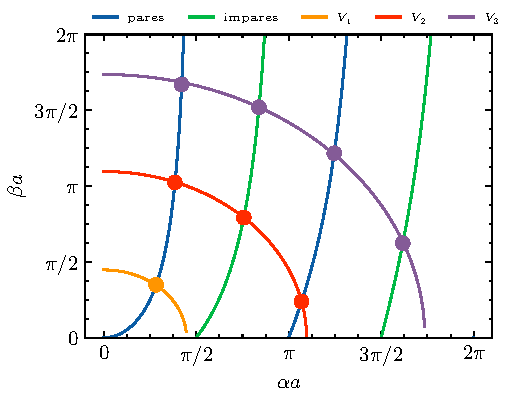
\includegraphics[width=0.5\linewidth]{media/slabgraphical.pdf}
\caption[Graphical solutions for TE modes.]{Graphical solutions for TE modes. A higher contrast $\Delta n = n_1-n_0$, results in a greater number of guided modes supported by the waveguide. \label{fig:graphTE}}
\end{figure}
After finding  $k_z$, we have everything needed to substitute into the expressions obtained for the components of the electromagnetic field. Figure \ref{fig:E-slab-graph} plots the spatial form of four modes, which correspond to the four purple points in Figure \ref{fig:graphTE}.
\begin{figure}[H]
	\centering
	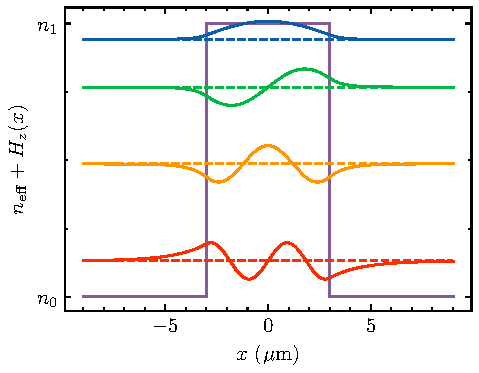
\includegraphics[width=0.5\linewidth]{media/TETMfields.pdf}
	\caption[Forma espacial de la componente longitudinal del campo magnético.]{ Spatial form of the longitudinal component of the magnetic field. \label{fig:E-slab-graph}}
\end{figure}

The cutoff condition in waveguides is equivalent to the energy no longer decaying in the region  $|x| > a$, meaning that $\beta a \to 0$ must hold.
Symmetric or even modes satisfy this condition when $\sin(V) = 0$, which implies $V = m \pi$, where $m$ is an integer. In particular, considering $m=0$  and sweeping  $n_1 \to n_0$, there are always at least two modes—one TE and one TM—as long as $n_1 > n_0$.  
Antisymmetric or odd modes, on the other hand, must satisfy $\cos(V) = 0$, which implies $V = (m\pi \pm \pi/2)$. From this condition, it follows that the first pair of excited modes ($m=0$) exists whenever $\lambda \le \lambda_c \equiv 4a\sqrt{n_1^2-n_0^2}$. Written compactly for the $m$-th mode:
\begin{align*}
	(\lambda_c)_m = \frac{4a}{m - 1} \sqrt{n_1^2 - n_0^2} \ ,
\end{align*}
which for $a=4 \text{ }\mu$m and $\Delta n = 5\times 10^{-4}$  implies a cutoff wavelength for the second mode of  $\lambda_c \approx 615 \text{ nm}$.
\section{Analytical solutions for circular optical fiber}
In the previous section, the simplest system in which dielectric waveguides can be discussed was studied. The next step in complexity involves circular waveguides. For this purpose, it will be considered that the refractive index varies radially according to:
\begin{equation}
	n( \rho ) = 
	\left\{\begin{matrix}
	n_1, \quad \text{if } \rho \le a
	\\
	n_0, \quad \text{if } \rho > a
	\end{matrix}\right.
	\ ,\nonumber
\end{equation}
where the tuple $(\rho, \phi, z)$ defines the cylindrical coordinates most appropriate for this problem.

When considering the longitudinal components $\Psi$ = $\{E_z, H_z\}$ of the electric and magnetic fields and using the method of separation of variables with $\Psi =  R(\rho)\Phi(\phi) e^{ik_z z} $,  equations (\ref{eqn:helmholz}) and (\ref{eqn:helmholzH}) take the form:
\begin{align}
	\left[\frac{\partial^2}{\partial \rho^2} + \frac{\partial}{\rho\partial \rho} + \frac{\partial^2}{\rho^2\partial \phi^2} +\left( k_0^2n^2 - k_z^2 \right)\right]  R(\rho)\Phi(\phi) = 0
	\nonumber
	\\
\rho^2\frac{d^2 R}{Rd\rho^2} + \rho\frac{dR}{Rd\rho} + \rho^2\left( k_0^2n^2 - k_z^2 \right) + \underbrace{\frac{d^2 \Phi}{\Phi d\phi^2}}_{-\ell^2} = 0
\nonumber
\end{align}
\vspace{-3em}
\begin{align}
\therefore \Phi(\phi) = A e^{i\ell\phi}
\nonumber
\end{align}
After imposing periodicity conditions  $\Phi(\phi)=\Phi(\phi + 2\pi)$, it necessarily follows that $\ell$ is an integer. Consequently, the equation for $R(\rho)$  is of the integer Bessel type. Therefore, seeking solutions such that $k_0^2 n_0^2 < \beta_z^2 < k_0^2 n_1^2$ and defining again $\alpha^2 \equiv k_0^2n_1^2 - k_z^2$ y $\beta^2\equiv k_z^2 - k_0^2n_0^2$ we have:
\begin{align}
	\frac{d^2 R}{d\rho^2} + \frac{1}{\rho}\frac{dR}{d\rho} + \left( k_0^2n^2 - k_z^2 -\frac{\ell^2}{\rho^2}\right)R  = 0
	\nonumber
	\\
	\therefore R(\rho) = 
	\left\{
	\begin{matrix}	
	C_1 J_\ell (\alpha\rho) + D_1 Y_\ell (\alpha\rho), \quad \text{if } \rho \le a  
	\\
	C_2 K_\ell (\beta\rho) + D_2 I_\ell (\beta\rho), \quad \text{if } \rho > a  
	\end{matrix}
	\right.
	\ . \nonumber
\end{align}
It is necessary to impose $D_1 = D_2 = 0$ or the solution to be finite at $\rho = 0$ and as $\rho \to +\infty$. That is, the radial part of the solution is:
\begin{align*}
 R(\rho) = 
	\left\{
	\begin{matrix}	
	C_1 J_\ell (\alpha\rho), \quad \text{if } \rho \le a  
	\\
	C_2 K_\ell (\beta\rho), \quad \text{if } \rho > a  
	\end{matrix}
	\right.
	\ . \nonumber
\end{align*}
In this case, to impose the continuity conditions on $\textbf{E}_{||} = E_\phi \boldsymbol{\hat{\phi}} + E_z \hat{\textbf{z}}$ and $\textbf{H}_{||}= H_\phi \hat{\boldsymbol{\phi}} + H_z \hat{\textbf{z}}$, it becomes necessary to relate the remaining field components to $E_z$​ and $H_z$​, for which equations (\ref{eqn:transversal}) are required.

Since 
\begin{equation*}
	\nabla_\perp \Psi =
	\left\{	
	\begin{matrix}
		\Psi_0^1\left[\boldsymbol{\hat{\rho}}\alpha J'_\ell (\alpha \rho) + i \boldsymbol{\hat{\phi}} \ell J_\ell (\alpha \rho)/\rho\right] e^{i\ell\phi} e^{i k_z z} \ , \quad \text{if } \rho \le a  
		\\
		\Psi_0^0\left[\boldsymbol{\hat{\rho}}\beta K'_\ell (\beta\rho) +i \boldsymbol{\hat{\phi}}\ell K_\ell (\alpha \rho)/\rho \right]e^{i\ell\phi} e^{i k_z z} \ , \quad \text{if } \rho > a  
	\end{matrix}
	\right.
\end{equation*}

Separating by components and substituting:
\begin{align*}
		H_z &=  e^{i\ell\phi}e^{i k_z z}
	  	 \left\{
		\begin{matrix}	  	 
	  	 H_0^1 J_\ell (\alpha \rho) \ , \quad \text{if } \rho \le a  
	  	 \\
	  	 H_0^0 K_\ell (\beta \rho) \ , \quad \text{if } \rho > a  
	  	 \end{matrix}
	  	 \right.	
		\\
	  	 H_r &= \frac{i e^{i\ell\phi}e^{i k_z z} }{k_0^2 n^2 - k_z^2}
	  	 \left\{
		\begin{matrix}	  	 
	  	  k_z \alpha H_0^1 J'_\ell (\alpha \rho) - i\omega \epsilon_0 n^2\ell E_0^1 J_\ell (\alpha \rho)/\rho \ , \quad \text{if } \rho \le a  
	  	 \\
	  	 k_z \beta H_0^0  K'_\ell (\beta \rho) - i\omega \epsilon_0 n^2\ell E_0^0 K_\ell (\beta \rho)/\rho \ , \quad \text{if } \rho > a  
	  	 \end{matrix}
	  	 \right.
	  	 \\
		H_\phi &= \frac{ie^{i\ell\phi} e^{i k_z z}}{k_0^2 n^2 - k_z^2}
		\left\{
		\begin{matrix}
			ik_z\ell H_0^1  J_\ell (\alpha \rho)/\rho + \omega \epsilon_0 n^2  \alpha E_0^1 J'_\ell (\alpha \rho) \ , \quad \text{if } \rho \le a  
			\\
			ik_z \ell H_0^0  K_\ell (\beta \rho)/\rho + \omega \epsilon_0 n^2 \beta E_0^0  K'_\ell (\beta \rho) \ , \quad \text{if } \rho > a  
		\end{matrix}
		\right.
		\\
		E_z &= e^{i\ell\phi} e^{i k_z z}
	  	 \left\{
		\begin{matrix}	  	 
	  	 E_0^1 J_\ell (\alpha \rho) \ , \quad \text{if } \rho \le a  
	  	 \\
	  	 E_0^0 K_\ell (\beta \rho) \ , \quad \text{if } \rho > a  
	  	 \end{matrix}
	  	 \right.	
		\\
	E_r &= \frac{i e^{i\ell\phi} e^{i k_z z} }{k_0^2 n^2 - k_z^2}
	  	 \left\{
		\begin{matrix}	  	 
	  	  k_z \alpha E_0^1 J'_\ell (\alpha \rho)+i\omega \mu_0 \ell H_0^1 J_\ell (\alpha \rho)/\rho \ , \quad \text{if } \rho \le a  
	  	 \\
	  	 k_z \beta E_0^0  K'_\ell (\beta \rho) +i\omega \mu_0 \ell H_0^0 K_\ell (\beta \rho)/\rho \ , \quad \text{if } \rho > a  
	  	 \end{matrix}
	  	 \right.
	\\
	E_\phi &= \frac{i e^{i\ell\phi} e^{i k_z z}}{k_0^2 n^2 - k_z^2}
		\left\{
		\begin{matrix}
			ik_z \ell E_0^1   J_\ell (\alpha \rho)/\rho -\omega \mu_0  \alpha H_0^1  J'_\ell (\alpha \rho) \ , \quad \text{if } \rho \le a  
			\\
			ik_z \ell E_0^0   K_\ell (\beta \rho)/\rho -\omega \mu_0 \beta H_0^0   K'_\ell (\beta \rho) \ , \quad \text{if } \rho > a  
		\end{matrix}
		\right.
\end{align*}
Then, imposing continuity in $z$ and $\phi$:
\begin{align}
	H_0^{1} J_\ell(\alpha a) &= H_0^{0} K_\ell (\beta a)
	\label{eqn:cont1}
	\\
	E_0^{1} J_\ell(\alpha a) &= E_0^{0} K_\ell (\beta a)
	\label{eqn:cont2}
	 \\
	 -\omega \epsilon_0 n_1^2  \alpha\beta^2 a E_0^1 J'_\ell (\alpha a)-ik_z\ell \beta^2 H_0^1  J_\ell (\alpha a)
	 &= \omega \epsilon_0 n_0^2 \alpha^2 \beta a E_0^0 K'_\ell (\beta a)+ik_z\ell \alpha^2H_0^0  K_\ell (\beta a)
	 \label{eqn:cont3}
	 \\
	 -ik_z \ell \beta^2 E_0^1   J_\ell (\alpha a) + \omega \mu_0  \alpha \beta^2 a H_0^1  J'_\ell (\alpha a) &=
	 ik_z \ell \alpha^2 E_0^0   K_\ell (\beta a) -\omega \mu_0  \alpha^2 \beta a H_0^0  K'_\ell (\beta a)
	 \label{eqn:cont4}
\end{align}
Seeking non-trivial solutions:
\begin{align*}
	\left|\begin{matrix}
		K_\ell(\beta a) & -J_\ell(\alpha a) & 0 & 0
		\\
		0 & 0 & K_\ell(\beta a) & -J_\ell(\alpha a)
		\\
		ik_z\ell \alpha^2 K_\ell (\beta a) & ik_z\ell\beta^2 J_\ell (\alpha a) & \omega \epsilon_0 n_0^2  \alpha^2 \beta a K'_\ell (\beta a) & \omega \epsilon_0 n_1^2  \alpha \beta^2 a J'_\ell (\alpha a)
		\\
		\omega \mu_0  \alpha^2 \beta a   K'_\ell (\beta a) &  \omega \mu_0  \alpha \beta^2 a J'_\ell (\alpha a) & -ik_z \ell \alpha^2 K_\ell (\beta a) &  -ik_z \ell \beta^2  J_\ell (\alpha a)
	\end{matrix}\right|
	=
0
\end{align*}
Finally, the transcendental equation satisfied by  $\alpha$, $\beta$ and $k_z$ is:
\begin{equation}
	\left( \frac{J_\ell'(\alpha a)}{\alpha a J_\ell(\alpha a)} + \frac{K_\ell'(\beta a)}{\beta a K_\ell(\beta a)} \right)\left( n_1^2\frac{J_\ell'(\alpha a)}{\alpha a J_\ell(\alpha a)} + n_0^2\frac{K_\ell'(\beta a)}{\beta a K_\ell(\beta a)} \right) = \ell^2 \left[ \left(\frac{1}{\alpha a}\right)^2 + \left(\frac{1}{\beta a}\right)^2 \right]^2 \left( \frac{k_z}{k_0} \right)^2 . \label{eqn:fiber_trascendental}
\end{equation}
Since, in principle, the values of $k_z$ are already determined by the equation above, it is possible to obtain two relations between $H_0^1$ and $E_0^1$:
\begin{align}
\frac{E_0^1}{H_0^1} &=  -\frac{i k_z \ell}{\omega\epsilon_0}\left[ \left(\frac{1}{\alpha a}\right)^2 + \left(\frac{1}{\beta a}\right)^2 \right]  \left[ n_1^2 \frac{J'_\ell(\alpha a)}{\alpha a J_\ell(\alpha a)} + n_0^2 \frac{K'_\ell(\beta a)}{\beta a K_\ell(\beta a)} \right]^{-1} \label{eqn:fiber_polarization_E},
\\
\frac{H_0^1}{E_0^1} &=  \frac{i k_z \ell}{ \omega\mu_0}\left[ \left(\frac{1}{\alpha a}\right)^2 + \left(\frac{1}{\beta a}\right)^2 \right]  \left[ \frac{J'_\ell(\alpha a)}{\alpha a J_\ell(\alpha a)} + \frac{K'_\ell(\beta a)}{\beta a K_\ell(\beta a)} \right]^{-1} \label{eqn:fiber_polarization_H}.
\end{align}
Taking the square root of the quotient of the equations: (\ref{eqn:fiber_polarization_E}) ans (\ref{eqn:fiber_polarization_H}) we have:
\begin{equation}
	\frac{E_0^1}{H_0^1} = i \sqrt{\frac{\mu_0}{\epsilon_0}} \frac{\sqrt{ \frac{J'_\ell(\alpha a)}{\alpha a J_\ell(\alpha a)} + \frac{K'_\ell(\beta a)}{\beta a K_\ell(\beta a)}}}{\sqrt{n_1^2 \frac{J'_\ell(\alpha a)}{\alpha a J_\ell(\alpha a)} + n_0^2 \frac{K'_\ell(\beta a)}{\beta a K_\ell(\beta a)}}} \ .
	\label{eqn:fiber_polarization_simplified}
\end{equation}
\subsection{TE and TM modes}
The simplest case to study is by imposing $\ell = 0$. Equation (\ref{eqn:fiber_trascendental}) implies:
\begin{align*}
	\frac{J'_{0}(\alpha a)}{\alpha a J_0(\alpha a)} + \frac{K'_0(\beta a)}{\beta a K_0(\beta a)}&=  0 \ , \quad \text{(TE modes)}
	\\
	n_1^2\frac{J'_{0}(\alpha a)}{\alpha a J_0(\alpha a)} + n_0^2 \frac{K'_0(\beta a)}{\beta a K_0(\beta a)} &= 0 \ , \quad \text{(TM modes)}
\end{align*}
from equation (\ref{eqn:fiber_polarization_simplified}), it is straightforward to note that the conditions for transverse modes imply that the longitudinal components become zero in the respective cases: $H_0^1 = 0$for TE and $E_0^1 = 0$ for TM.

The cutoff conditions occur when $\beta a \to 0$. Using the asymptotic expressions for Bessel functions with small arguments and their recurrence relations, we have:
\begin{align*}
	\frac{\alpha a J_0(\alpha a)}{J_1(\alpha a)}  = -\frac{\beta a K_{0}(\beta a)} {K_1(\beta a)} \approx (\beta a)^2\ln\left(\frac{\beta a e^\gamma}{2}\right) \to 0 \ ,
\end{align*}
thus it becomes necessary that $\left. J_0(\alpha a)\right|_{\alpha a \to V} = 0$. Denoting $x_{0,m}=$ 2.405,  5.520,  8.654, $\cdots$ as the  $m$-th zero of the function $J_0(x)$, the cutoff wavelength is given by:
\begin{equation}
(\lambda_c)_{0,m} = 2\pi a \frac{\sqrt{n_1^2 - n_0^2}}{x_{0,m}} \ , \quad\text{(TE and TM modes)},
\end{equation} 
which translates to a cutoff wavelength of: $\lambda_c\approx 616$ nm for the same parameters as in the section \ref{cap:slab}, $a=4 \text{ }\mu$m y $\Delta n = 5\times 10^{-4}$ . Contrary to the case of slab waveguides, in optical fibers it is necessary to be below a non-zero maximum cutoff threshold $(\lambda_c)_{0,1}$ for TE or TM modes to exist. As will be seen later, this is because purely transverse modes correspond to excited modes: the fundamental mode is hybrid.


%\begin{figure}[H]
%	\centering
%	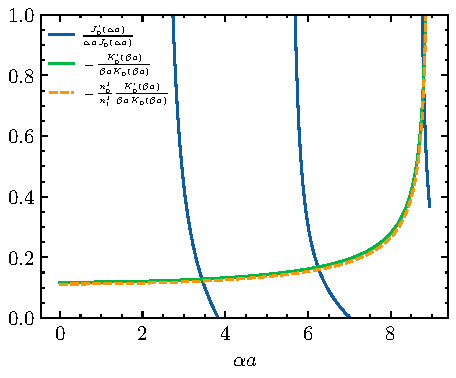
\includegraphics[width=0.7\linewidth]{media/fibergraphical}
%\end{figure}

\subsection{HE and EH modes}
Interpreting (\ref{eqn:fiber_trascendental}) as a quadratic equation in $J_\ell'(\alpha a)/\alpha a J_\ell(\alpha a)$:
\begin{align*}
	\frac{J_\ell'(\alpha a)}{\alpha a J_\ell(\alpha a)} &= -\left(\frac{n_1^2+n_0^2}{2n_1^2}\right) \frac{K_\ell'(\beta a)}{\beta a K_\ell(\beta a)}\pm\sqrt{\left(\frac{n_1^2-n_0^2}{2n_1^2}\right)^2\left(\frac{K_\ell'(\beta a)}{\beta a K_\ell(\beta a)}\right)^2+ \left( \frac{ k_z \ell}{ k_0 n_1} \right)^2\left[ \left(\frac{1}{\alpha a}\right)^2 + \left(\frac{1}{\beta a}\right)^2 \right]^2 }
\end{align*}

If the recurrence relations of the Bessel functions $J_\ell(r)$,are used, it is possible to obtain two types of solutions that are usually called HE and EH due to the longitudinal field with greater relative value:
\begin{align}
		\frac{J_{\ell-1}(\alpha a)}{\alpha a J_\ell(\alpha a)} &= -\left(\frac{n_1^2+n_0^2}{2n_1^2}\right) \frac{K_\ell'(\beta a)}{\beta a K_\ell(\beta a)}+\frac{\ell}{(\alpha a)^2}-\sqrt{\Delta} \ , \quad \text{(HE modes)}
		\label{eqn:HE}
	\\
		\frac{J_{\ell+1}(\alpha a)}{\alpha a J_\ell(\alpha a)} &= \left(\frac{n_1^2+n_0^2}{2n_1^2}\right) \frac{K_\ell'(\beta a)}{\beta a K_\ell(\beta a)}+\frac{\ell}{(\alpha a)^2}-\sqrt{\Delta} \ , \quad \text{(EH modes)}
		\label{eqn:EH}
		\\
		\Delta &= \left(\frac{n_1^2-n_0^2}{2n_1^2}\right)^2\left(\frac{K_\ell'(\beta a)}{\beta a K_\ell(\beta a)}\right)^2+ \left( \frac{ k_z \ell}{ k_0 n_1} \right)^2\left[ \left(\frac{1}{\alpha a}\right)^2 + \left(\frac{1}{\beta a}\right)^2 \right]^2 \ . \nonumber
\end{align}
For $\ell = 0$,  the relations obtained for the TE$_m$ (HE$_{0m}$) and TM$_m$ (EH$_{0m}$). For $\ell \neq 0$ it becomes necessary to consider the asymptotic expressions of the Bessel functions when $\beta a \to 0$ and $\alpha a \to V$:
\begin{align*}
	\frac{K'_\ell (x)}{xK_\ell (x)} &= -\frac{K_{\ell-1} (x)}{xK_\ell (x)}-\frac{\ell}{x^2}\approx \left\{\begin{matrix}
	\ln(xe^\gamma/2)-\frac{1}{x^2} \quad\text{si }\ell = 1
	\\
	-\frac{
	1}{2(\ell-1)}-\frac{\ell}{x^2}\quad \text{si }\ell > 1
	\end{matrix}\right. .
\end{align*}
The case $\ell=1$ is of special interest. The condition for HE modes is developed as:
\begin{align*}
	\frac{\alpha a J_1(\alpha a)}{J_0(\alpha a)} &= \left\{\left(\frac{n_1^2+n_0^2}{2n_1^2}\right) \left[ \ln\left(\frac{2}{e^\gamma \beta a}\right)+\frac{1}{(\beta a)^2} \right]+\frac{1}{(\alpha a)^2}-\sqrt{\Delta}\right\}^{-1} \to 0 \ .
\end{align*}
It is sufficient to consider the function $J_1(\alpha a)|_{\alpha a \to V} = 0$. On the other hand, the EH condition eliminates the zero $x=0$ from the ratio $\frac{\alpha aJ_1(\alpha a)}{J_2(\alpha a)}$ which causes it to be "out of phase" relative to the HE condition. Using reasoning similar to the $\ell =0$, case, the cutoff conditions are:
\begin{align*}
	(\lambda_c)_{1,m} &= 2\pi a \frac{\sqrt{n_1^2 - n_0^2}}{x_{1,m}} \ ,  \quad \left(\text{HE modes}_{1m}\right)
	\\
	(\lambda_c)_{1,m} &= 2\pi a \frac{\sqrt{n_1^2 - n_0^2}}{x_{1,m+1}} \ , \quad \left(\text{EH modes}_{1m}\right)
\end{align*}
with $x_{1,m}=$ 0, 3.832,  7.016, 10.173, $\dots$. In particular, the $\text{HE}_{11}$ mode always exists. The next largest finite cutoff wavelengths are $\lambda_c \approx 252$ nm for the $\text{HE}_{12}$ and $\text{EH}_{11}$ modes.

The case $\ell \ge 2$ has a different development due to the asymptotic forms involved and will not be relevant for this thesis. However, they are included in Figure \ref{fig:vortices} for completeness.
\begin{figure}[H]
	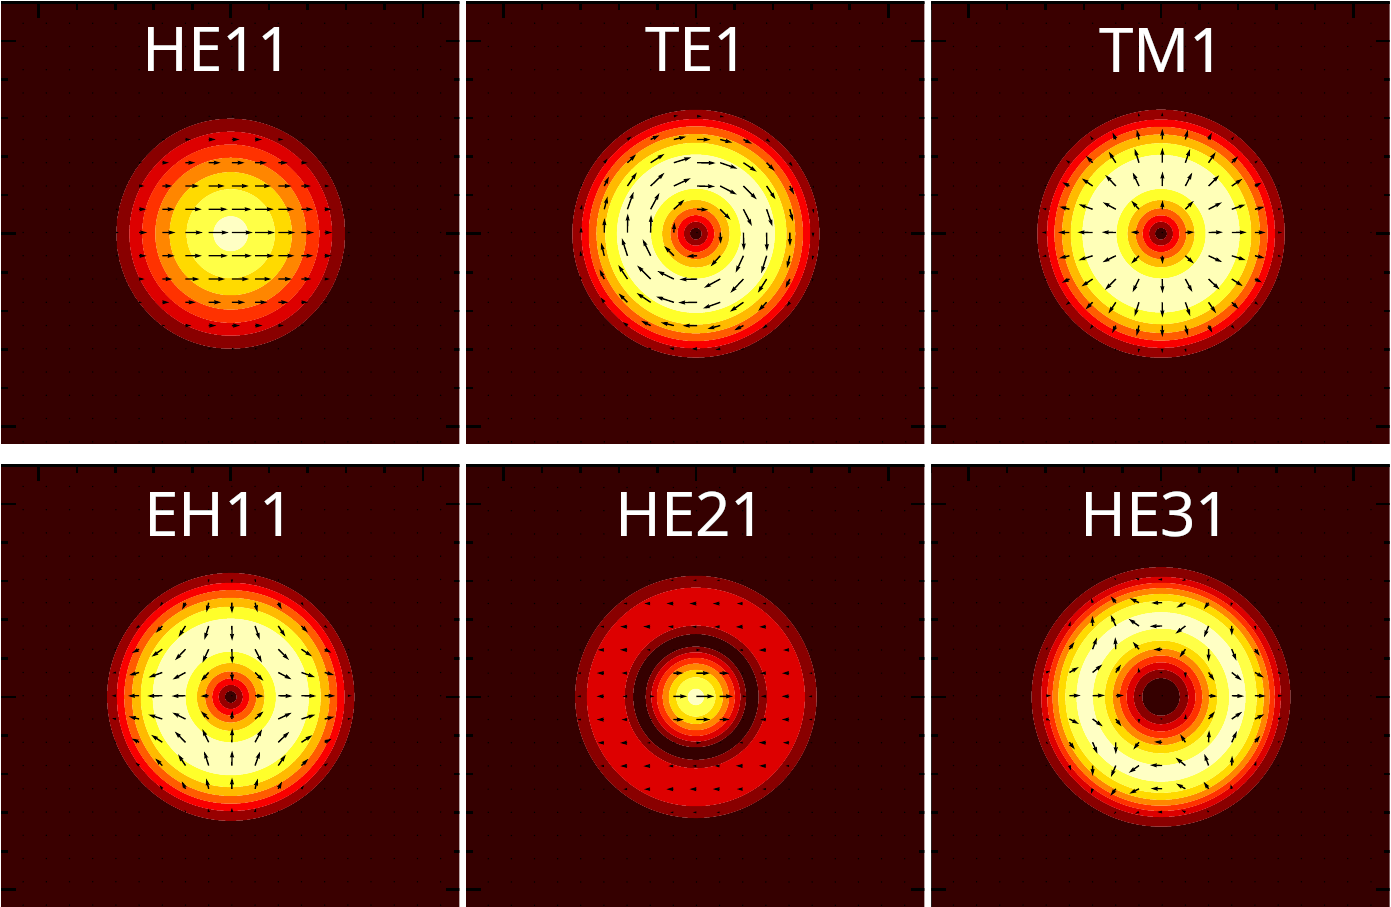
\includegraphics[width=\linewidth]{media/OAM_analitic}
		\caption{First guided normal modes for a circular waveguide or optical fiber. \label{fig:vortices}}
\end{figure}

\section{Normal modes in waveguides}

If the waveguide structure does not vary in the  \( \hat{\textbf{z}} \)direction, the solution for the electric field can be written, by separation of variables, as a plane wave of the form \( \textbf{E}(\textbf{r}) = \textbf{E}_\nu(x, y) e^{i\beta_\nu z} \). In turn, it is convenient to separate the Laplacian operator as \( \nabla^2 = \nabla_\perp^2 + \frac{\partial^2}{\partial z^2} \). 

Defining the operator \( D_{ij} \) such that  \( D_{ij} E_j \equiv \partial_i\left(\frac{\partial_j n^2}{n^2}E_j \right) \), he transverse part of the Helmholtz equations (\ref{eqn:helmholz}) can be written as:
\begin{align}
	\begin{pmatrix}
		\nabla_\perp^2  + k_0^2n^2 + D_{xx} & D_{xy} 
		\\
		D_{yx}  & \nabla_\perp^2  + k_0^2n^2 + D_{yy} 
	\end{pmatrix}
	\begin{pmatrix}
		E_x
		\\
		E_y
	\end{pmatrix}
	=
	\beta_\nu^2 
	\begin{pmatrix}
		E_x
		\\
		E_y
	\end{pmatrix} \ . \label{eqn:eigenfield}
\end{align}

Equation (\ref{eqn:eigenfield}) constitutes an eigenvalue problem for \( \beta_\nu^2 \), whose eigenfunctions \( \textbf{E}_\nu^\perp(x,y) \) d describe the transverse profiles of the guided modes. In general, this is a coupled vectorial second-order system, whose resolution requires numerical techniques. However, in the \textit{weak guidance} regime, where the refractive index varies slightly relative to a homogeneous background  \( n_0 \), the system can be decoupled and treated as a scalar problem for a dominant component of the electric field\footnote{see \ref{sec:orto}.}.

Under this approximation, quasi-transverse modes are typically considered, where the electric field is primarily polarized in a fixed direction (for example, \( E_y \)), and the Helmholtz equation reduces to:
\begin{equation}
	\left[\nabla_\perp^2 + k_0^2 n^2(x,y) \right] \phi_\nu(x,y) = \beta_\nu^2 \phi_\nu(x,y) \ ,
\end{equation}
where \( \phi_\nu(x,y) \) represents the transverse field profile. This approximation is valid for many experimental geometries, especially when the light is linearly polarized and the index variations do not induce coupling between orthogonal polarizations.

The modes obtained from this equation allow for the calculation of propagation constants \( \beta_\nu \), spatial field profiles \( \phi_\nu(x,y) \), and other relevant quantities such as confinement factors or group velocities. Furthermore, these modes serve as a basis for subsequent numerical methods, such as Eigenmode Expansion (EME) or Coupled-Mode Theory (CMT), used to describe the dynamics in photonic lattices.
\section{Coupled-Mode Theory \label{cap:CMTteo}}
\subsection{Derivation from a Variational Principle}

From equations (\ref{eqn:EfieldH}) and (\ref{eqn:HfieldE}), it is possible to express the propagation constant $k_z$ in terms of the Poynting vector $\textbf{S} = \frac{1}{2} \text{Re}\{\textbf{E} \times \textbf{H}^*\}$, following a derivation analogous to that presented in \citep{haus_coupled-mode}. 
\begin{equation}
	k_z = \frac{
		\frac{1}{4i} \iint \left[
		\left(-\nabla_\perp \times \textbf{E} + i\omega \mu_0 \textbf{H}\right) \cdot \textbf{H}^* 
		+ \left(\nabla_\perp \times \textbf{H} + i\omega \varepsilon_0 n^2 \textbf{E}\right) \cdot \textbf{E}^*
		\right] dxdy
	}{
		\frac{1}{4} \iint \left( 
		\textbf{E} \times \textbf{H}^* + \textbf{E}^* \times \textbf{H}
		\right) \cdot \hat{\textbf{z}} \, dxdy
	} \ . 
	\label{eqn:kzprevar}
\end{equation}
When proposing a solution in the form of a superposition of modes from the individual waveguides, such as:
\begin{align*}
	\textbf{E} &= \sum_i a_i \textbf{e}_i \ , \quad \textbf{H} = \sum_i a_i \textbf{h}_i \ ,
\end{align*}
where $a_i$ represents the amplitude of the $i$-th mode, the coefficients remain undetermined but subject to minimizing the expression for $k_z$. Substituting these expansions into (\ref{eqn:kzprevar}), a simplified expression for the propagation constant of the system $k_z$ is obtained:
\begin{align*}
	(\textbf{E}\times\textbf{H}^* + \textbf{E}^*\times\textbf{H})\cdot\hat{\textbf{z}} 
	&= \sum_{ij} a_i^* \left( \textbf{e}_j \times \textbf{h}_i^* + \textbf{e}_i^* \times \textbf{h}_j \right) \cdot \hat{\textbf{z}} \, a_j 
	\equiv \sum_{ij} a_i^* p_{ij} a_j \ .
\end{align*}
The integrand of the numerator is expanded as:
\begin{align*}
	\text{integrand of the numerator} &= i\sum_{ij} \Big[ a_i^* k_z^j (\hat{\textbf{z}}\times\textbf{e}_j )\cdot\textbf{h}_i^* a_j  + a_j \left(\omega \varepsilon_0 (n^2-n_j^2) \textbf{e}_j - k_z^j \hat{\textbf{z}}\times\textbf{h}_j \right) \cdot \textbf{e}_i^* a_i^* \Big] \ , \\
	&= i\sum_{ij} a_i^* \left[ k_z^j p_{ij} + \omega \varepsilon_0(n^2-n_j^2) \textbf{e}_j \cdot \textbf{e}_i^* \right] a_j \ ,
\end{align*}
where $k_z^j$ is the propagation constant of the $j$-th isolated mode\footnote{in general, $k_z \neq k_z^j$.}. 

Defining the following fundamental quantities:
\begin{align}
	P_{ij} &\equiv \frac{1}{4} \iint \left( \textbf{e}_j \times \textbf{h}_i^* + \textbf{e}_i^* \times \textbf{h}_j \right) \cdot \hat{\textbf{z}} \ , dxdy, \label{eqn:pij-ori} \\
	&= \frac{1}{4 \omega \mu_0} \iint \Big[ 
	(k_z^i + k_z^j) \left( \textbf{e}_i^* \cdot \textbf{e}_j - e_{z,i}^* e_{z,j} \right)  + i \left( \textbf{e}_i^* \cdot \nabla_\perp e_{z,j} + \textbf{e}_j \cdot \nabla_\perp e_{z,i}^* \right) \Big] dxdy \ , \label{eqn:pij-simpli} \\
	H_{ij} &\equiv P_{ij} k_z^j + \frac{\omega \varepsilon_0}{4} \iint (n^2-n_j^2) \textbf{e}_j \cdot \textbf{e}_i^* \, dxdy \ , \label{eqn:hij}
\end{align}
the expression (\ref{eqn:kzprevar}) for the propagation constant $k_z$ can be written compactly as a Rayleigh-Ritz quotient:
\begin{equation}
	k_z = \frac{\sum_{ij} a_i^* H_{ij} a_j}{\sum_{ij} a_i^*P_{ij} a_j} \ .
\end{equation}
Differentiating with respect to $a_k^*$ to optimize the value of $k_z$ yields:
\begin{align}
	\frac{\partial k_z}{\partial a_k^*} &= \frac{\sum_{ij} H_{ij} a_j \delta_{ik}}{\sum_{ij} a_i^*P_{ij} a_j} - \frac{\left(\sum_{ij} a_i^* H_{ij} a_j\right) \left( 
	\sum_{ij} \delta_{ik} P_{ij} a_j \right) }{\left(\sum_{ij} a_i^*P_{ij} a_j\right)^2} = \frac{\sum_{j} \left(H_{jk}  - k_z P_{kj} \right) a_j}{\sum_{ij} a_i^* P_{ij}a_j} \overset{!}{=} 0 \ .
\end{align}
Recovering $k_z \to -i\frac{\partial}{\partial z}$, the equations for $N$ non-orthogonal coupled modes are obtained:
\begin{equation}
	-i \sum_{j} P_{kj} \frac{d a_j}{dz} ´= \sum_{j} H_{kj} a_j \ , \text{ with }k=1,2,\cdots,N \ . \label{eqn:non-ortho-CMT-eqs}
\end{equation}
Clearly, from the expression (\ref{eqn:pij-ori}) for $P_{ij}$, Hermiticity is satisfied. At first glance, it may seem that $H_{ij}$ is not Hermitian, but let us see that it indeed is. To do this, it suffices to consider the difference $H_{ij} - H_{ji}^*$ and note that it vanishes:
\begin{align*}
 H_{ij} - H_{ji}^* &= P_{ij} k_z^j - P_{ji}^* k_z^i  + \frac{\omega \varepsilon_0}{4} \iint(n_i^2-n_j^2) \textbf{e}_i^* \cdot \textbf{e}_j dxdy
\\
&= \frac{1}{4} \iint (k_z^j-k_z^i)( \textbf{e}_j \times  \textbf{h}_i^* + \textbf{e}_i^* \times  \textbf{h}_j  )\cdot\hat{\textbf{z}} + \omega\varepsilon_0 (n_i^2-n_j^2) \textbf{e}_j \cdot \textbf{e}_i^* dxdy
\\
&= \frac{1}{4} \iint \left( i\nabla_\perp \times \textbf{e}_j +\omega\mu_0 \textbf{h}_j \right) \cdot \textbf{h}_i^* - \left( i\nabla_\perp \times \textbf{h}_j  - \omega\varepsilon_0n_j^2 \textbf{e}_j \right) \cdot \textbf{e}_i^*dxdy
\\
&- \frac{1}{4} \iint \left( i\nabla_\perp \times \textbf{e}_i^* +\omega\mu_0 \textbf{h}_i^*\right) \cdot \textbf{h}_j + \left(i\nabla_\perp \times \textbf{h}_i^*  + \omega\varepsilon_0n_i^2 \textbf{e}_i^* \right) \cdot \textbf{e}_jdxdy
\\
&+\frac{\omega\varepsilon_0}{4}\iint  \left(n_i^2-n_j^2\right) \textbf{e}_j \cdot \textbf{e}_i^* dxdy
\\
&= \frac{i}{4} \iint \left(\nabla_\perp\times\textbf{e}_j\right) \cdot \textbf{h}_i^*  -\left(\nabla_\perp\times\textbf{h}_j\right) \cdot \textbf{e}_i^* + \left(\nabla_\perp\times\textbf{e}_i^*\right) \cdot \textbf{h}_j - \left(\nabla_\perp\times\textbf{h}_i^*\right) \cdot \textbf{e}_j dxdy
\\
&= \frac{i}{4} \iint \nabla_\perp\cdot\left(\textbf{e}_j \times \textbf{h}_i^* +\textbf{e}_i^* \times \textbf{h}_j\right) dxdy =
\frac{i}{4} \oint_C \left(\textbf{e}_j \times \textbf{h}_i^* +\textbf{e}_i^* \times \textbf{h}_j\right) \cdot \hat{\textbf{n}} ds
\\
&=
0 \ ,
	\end{align*}
where it has been used that the fields must decay to zero at infinity. Equations (\ref{eqn:non-ortho-CMT-eqs}) can be derived from a Principle of Least Action after defining the discrete field Lagrangian $L$ of the Schrödinger type:
\begin{equation}
	L = -\sum_{ij}  a_i^*\left(i  P_{ij} \frac{d }{dz} + H_{ij}  \right)a_j \ .
\end{equation}
The generalized momenta of this Lagrangian are $\Pi_k=\frac{\partial L}{\partial \dot{a_k}} = -i\sum_{j} a_j^* P_{jk}$, so the associated Hamiltonian $H$ is:
\begin{equation}
H = \sum_{j} \Pi_j \dot{a_j} - L = \sum_{ij} -ia_i^* P_{ij} \dot{a_j} + a_i^*\left(i  P_{ij} \frac{d a_j}{dz} + H_{ij} a_j \right) = \sum_{ij} a_i^* H_{ij} a_j \ .
\end{equation}
Since the Lagrangian does not depend explicitly on $z$, the Hamiltonian $H$ is a conserved quantity. Varying the Lagrangian yields:
\begin{align*}
	\delta L &= \sum_{ij} \frac{\partial L}{\partial a_j} \delta a_{j} +  \frac{\partial L}{\partial {a}_{i}^*} \delta {a}_{i}^* + \ \frac{\partial L}{\partial \dot{a}_{j}} \delta \dot{a}_{j} + \frac{\partial L}{\partial \dot{{a}}_{i}^*} \delta \dot{{a}}_{i}^*
	\\
	&= \sum_{ij} \left( \frac{\partial L}{\partial a_{j}} - \frac{d}{dz}\frac{\partial L}{\partial \dot{a}_{j}} \right)\delta a_{j} + \left( \frac{\partial L}{\partial {a}_{i}^*} - \frac{d}{dz}\frac{\partial L}{\partial  \dot{{a}}_{i}^*} \right)\delta {a}_{i}^* + \frac{d}{dz}\left(\frac{\partial L}{\partial \dot{a}_{j}}\delta a_{j} +  \frac{\partial L}{\partial \dot{{a}}^*_{i}}\delta {a}_{i}^*\right)
	\\	
	&\implies  \frac{d}{dz} \sum_{ij}\left(\frac{\partial L}{\partial \dot{a}_{j}}\delta a_{j} +  \frac{\partial L}{\partial \dot{{a}}_{i}^*}\delta {a}_{i}^*\right) = 0 \ .
\end{align*}
The pair of transformations associated with the unitary group U(1), $a_j\to a'_j = e^{i\phi}a_j$, ${a}_i^* \to {a'}_i^* = e^{-i\phi}{a}_i^*$ leave the Lagrangian invariant. If an infinitesimal variation $\phi \ll 1$ is taken, then $\delta a_j = i\phi a_j$ and $\delta {a}_i^* = -i\phi {a}_i^*$, is taken, then $P$, which is identified with the total power of the system and is directly related to the Poynting vector, is:
\begin{equation}
	P = \sum_{ij} a_i^* P_{ij} a_j = \iint \textbf{S} \cdot \hat{\textbf{z}} dxdy \ .  \label{eqn:power}
\end{equation}
Thus, there are two conserved quantities in the dynamics, $H$ y $P$, which will be useful for verifying the validity of numerical solutions to equation (\ref{eqn:non-ortho-CMT-eqs}).

\subsection{TE Dimer in Slab-Type Waveguides}
Using the equations for the transverse components (\ref{eqn:transverse}) in the case of fundamental TE modes (\ref{eqn:TEanti}), we have:
\begin{align*}
	\textbf{e}_{j\perp} &= \hat{\textbf{y}}\frac{i\omega\mu_0 H_{a1}}{k_0^2n_j^2 - (k_z^j)^2}\left\{ \begin{matrix}
-\alpha \cos(\alpha (x-x_j)), &|x-x_j|\le a
\\
\beta\sin(\alpha a) e^{-\beta(|x-x_j|-a)}, &|x-x_j| > a
\end{matrix}\right. \ ,
\\
\textbf{h}_{j\perp} &= \hat{\textbf{x}}\frac{ik_z^j H_{a1}}{k_0^2n_j^2 - (k_z^j)^2}\left\{ \begin{matrix}
\alpha \cos(\alpha (x-x_j)), &|x-x_j|\le a
\\
-\beta\sin(\alpha a) e^{-\beta(|x-x_j|-a)}, &|x-x_j| > a
\end{matrix}\right. \ ,
\end{align*} with $x_j=jd$, $d\ge 2a$ and $L=\int dy$. The off-diagonal elements have the form:
\begin{align*}
	\left(\textbf{e}_{j\perp}\times\textbf{h}_{i\perp}^*\right)\cdot \hat{\textbf{z}}
	&=
	\frac{k_z^i \omega \mu_0 H_{a1}^2 \beta\sin(\alpha a)}{(k_0^2n_j^2 - k_z^2)(k_0^2n_i^2 - k_z^2)}
	\left\{
	\begin{matrix}
		 \alpha\cos(\alpha(x-x_i))e^{-\beta(|x-x_j|-a)}, & |x-x_i| \le a
		\\
		i \leftrightarrow j, & |x-x_j| \le a
		\\
		\beta \sin(\alpha a)e^{-\beta (|x-x_i|+|x-x_j|-2a)}, & \text{otherwise}
	\end{matrix}
	\right. \ ,
\\
	P_{ij} &= \frac{L k_z^i k_0  \mu_0 c H_{a1}^2 \sin^2(\alpha a)e^{-\beta d}e^{\beta a}}{2\beta} \left[\frac{e^{-\beta a} + \beta (d-2a)e^{\beta a}}{\beta^2} - \frac{2\cosh(\beta a)}{\alpha^2+\beta^2} \right] \ ,
\\
	\tilde{H}_{ij} &\equiv H_{ij} - P_{ij} k_z^j = \frac{L k_0    \mu_0 c H_{a1}^2 }{2 \beta }  \sin^2(\alpha a)e^{2\beta a} e^{-\beta d} \ .
\end{align*}
The diagonal elements have the form:
\begin{align*}
	\left(\textbf{e}_{j\perp}\times\textbf{h}_{j\perp}^*\right)\cdot \hat{\textbf{z}}&=\frac{k_z^j\omega\mu_0 H_{a1}^2}{(k_0^2n_j^2-k_z^2)^2} \left\{ \begin{matrix}
\alpha^2\cos^2(\alpha (x-x_j)), & |x-x_j| \le a
\\
\beta^2 \sin^2(\alpha a) e^{2\beta a} e^{-2\beta|x-x_j|}, & |x-x_j|>a
\end{matrix}\right. \ ,
\\
	P_{jj} &= \frac{L k_z^j  k_0 \mu_0 c H_{a1}^2  a}{2 \alpha^2} \left[1 + \frac{\sin^2(\alpha a)}{a \beta^3 } k_0^2 \left( n_1^2 - n_0^2 \right) \right] \ ,
\\
	\tilde{H}_{jj} &\equiv H_{jj} - P_{jj} k_z^j =
	\frac{L k_0^3  \mu_0 c H_{a1}^2 \sin^2(\alpha a)e^{2\beta a}e^{-2\beta d}}{4 \beta^3 } (n_1^2-n_0^2) \sinh(2\beta a) \ .
\end{align*}
The dynamics is governed by the coupled system of equations (\ref{eqn:non-ortho-CMT-eqs}), which, after pre-multiplying by the inverse of the matrix $P_{ij}$, takes the compact form:
\begin{align*}
	-i\frac{d}{dz}\begin{pmatrix}
	a_1
	\\
	a_2
	\end{pmatrix} &= 	
	\begin{pmatrix}
	\tilde{k} & C
	\\
	C & \tilde{k}
	\end{pmatrix}
	\begin{pmatrix}
	a_1
	\\
	a_2
	\end{pmatrix} \ ,
\end{align*}
with, for example, $\tilde{k}\equiv k_z^{\text{TE}} + \delta k$, $k_z^{\text{TE}} \sim 1.3\times10^5 \text{ cm}^{-1}$, $C\equiv \frac{P_{ii} \tilde{H}_{ij}  -P_{ij}\tilde{H}_{ii}}{P_{ii}^2-P_{ij}^2} \sim 1\text{ cm}^{-1}$ and $\delta k \equiv \frac{P_{ii} \tilde{H}_{ii} -P_{ij}\tilde{H}_{ij}}{P_{ii}^2-P_{ij}^2} \sim -0.02\text{ cm}^{-1}$ for $\lambda = 730$ nm, $n_1 = n_0 + 4\times10^{-4}$ and a distance between waveguides of $d = 18 $ $\mu$m. The matrix $\hat{P}^{-1}\hat{H}$ can be written in terms of the Pauli matrices as $\tilde{k}I + C\sigma_x $, which allows using their properties to solve the system dynamics:
\begin{align*}
	\begin{pmatrix}
	a_1(z)
	\\
	a_2(z)
	\end{pmatrix}
	=
	e^{{i\left[\tilde{k}I + C\sigma_x\right]z }}	\begin{pmatrix}
	a_1(0)
	\\
	a_2(0)
	\end{pmatrix}
	=
	e^{i\tilde{k}z}
	\begin{pmatrix}
	\cos(Cz) & i\sin(Cz)
	\\
	i\sin(Cz) & \cos(Cz)
	\end{pmatrix}
	\begin{pmatrix}
	a_1(0)
	\\
	a_2(0)
	\end{pmatrix} \ .
\end{align*}
One way to experimentally determine the coupling value $C$ is by individually exciting one mode. With this, the ratio between the powers $|a_1(z)|^2$ and $|a_2(z)|^2$ allows solving for the coupling given a known propagation distance $z=L<\frac{\pi}{2C}$:
\begin{equation}
	C = \frac{1}{L}\tan^{-1}\left( \left|\frac{a_2(L)}{a_1(L)}\right|^2 \right) \ . \label{eqn:coupling-simp}
\end{equation}
\subsection{Bands and Topology: Photonic Su-Schrieffer-Heeger Lattice}
Although it is possible to reformulate Maxwell's equations as an eigenvalue problem in analogy with quantum mechanics to establish an analogue to Bloch's theorem \cite{joannopoulos_photonic_2008}, the Hermitian matrix $\hat{C}\equiv\hat{P}^{-1}\hat{H}$ from equation (\ref{eqn:non-ortho-CMT-eqs}) provides sufficient justification to invoke it: It is possible to express the solutions of the system in a quasimomentum basis whose periodicity matches that of the matrix $\hat{C}$.
To illustrate this, the celebrated Su-Schrieffer-Heeger (SSH) model will be used, which is one of the simplest systems exhibiting \textit{topological edge states} \cite{ssh, ssh-photonic, topological-photonics}. Originally developed to explain the formation of localized electronic states in polyacetylene, it involves considering only two types of coupling: one strong (double bond) and one weak (single bond). In terms of Solid State Physics, it corresponds to a one-dimensional lattice with a two-site basis, whose modal amplitudes are denoted $a_n$ and $b_n$. Figure \ref{fig:ssh-model} illustrates the model to be studied, which corresponds to the following Hamiltonian $H$. 
\begin{equation*}
	H = \sum_n \left( t b_n^*a_n + t'  a_{n+1}^*b_n  + c.c. \right) \ .
\end{equation*}
\begin{figure}[h]
\centering
	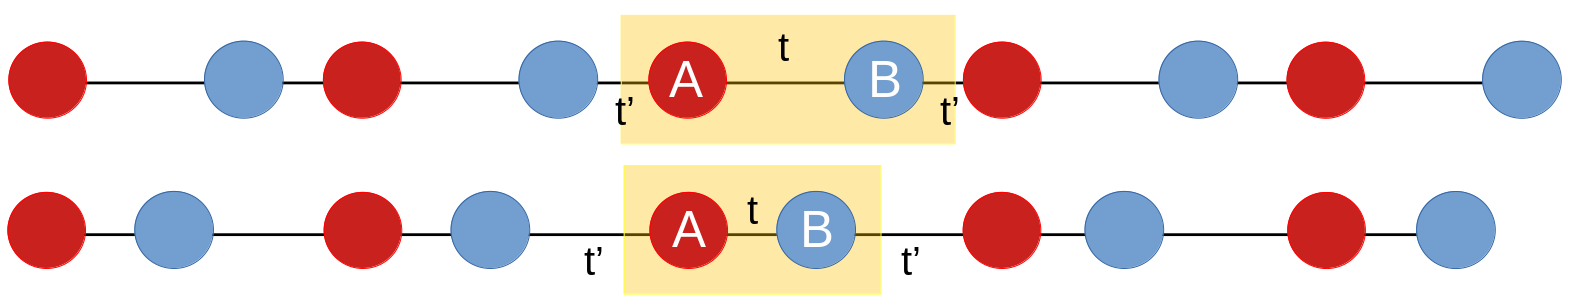
\includegraphics[width=\linewidth]{media/ssh-model.png}
	\caption[Schematic of the SSH model.]{Schematic of the SSH model. The unit cell is enclosed in yellow, where sites A and B and the intracell (intercell) coupling $t$ ($t'$) are distinguished. Two different configurations are shown. \label{fig:ssh-model}}
\end{figure}
Under periodic boundary conditions (Born–von Karman), it is possible to diagonalize the Hamiltonian in the Bloch basis with $a_n = \frac{1}{\sqrt{N}}\sum_k a_k e^{iknd}$, $b_n = \frac{1}{\sqrt{N}}\sum_k b_k e^{iknd}$ as follows:
\begin{align*}
	H &= \frac{1}{N}\sum_n \sum_{k k'} \left[\left(t + t' e^{ikd}\right) a_k b_{k'}^* e^{i(k-k')nd}  + \left(t  + t' e^{-ikd}\right) a_k^* b_{k'} e^{-i(k-k')nd} \right]
	\\
	&=  \sum_k 
	\begin{pmatrix}
		a_k^* & b_k^*		
	\end{pmatrix}
	\underbrace{
	\begin{pmatrix}
		0 & t+ t'e^{-ikd}
		\\
		t+ t'e^{ikd} & 0
	\end{pmatrix}}_{\hat{H}(k)}
	\begin{pmatrix}
		a_k
		\\
		b_k		
	\end{pmatrix},
\end{align*}
where it has been used that $$\frac{1}{N}\sum_n e^{i(k-k')nd} = \left\{\begin{matrix} \frac{N}{N}=1, &\text{ if } k = k'
\\ \frac{1}{N}\frac{1-\cancelto{1}{e^{i(k-k')Nd}}}{1-e^{i(k-k')d}}e^{i(k-k')d}=0, &\text{ if } k\neq k'
\end{matrix}\right. =\delta_{kk'},$$ since $k, k' \in  \left\{\frac{2\pi l}{Nd}, l=0,\pm 1, \dots , \pm \frac{N}{2}\right\}$ belong to the 1D reciprocal lattice. The spectrum of $\hat{H}(k)$ is $\lambda_k = \pm\sqrt{t^2+t'^2+2tt'\cos(kd)}$, which would seem to indicate that the system is symmetric between $t$ y $t'$. However, the picture is not complete without the eigenvectors of $\hat{H}(k)$, $\textbf{v}_\pm =\frac{1}{\sqrt{2}} \begin{pmatrix} \pm e^{-i\phi(k)} \\  1 \end{pmatrix}$, with $\phi(k)=\tan^{-1}\left(\frac{t'\sin(kd)}{t+t'\cos(kd)}\right)$. If the vector $\textbf{d}(k) \equiv \begin{pmatrix}t+t'\cos(kd) \\ t'\sin(kd) \\ 0 \end{pmatrix}$ is defined, it is possible to write the Hamiltonian $\hat{H}(k)$ in terms of the Pauli matrices as $\hat{H}(k) = \textbf{d} \cdot \bm{\sigma} = d_x\sigma_x + d_y\sigma_y$. This vector $\textbf{d}(k)$ is a vectorial representation of the $2\times2$ bulk Hamiltonian in momentum space. The phase $\phi(k)$ is related to the angle formed by the projection of the vector $\textbf{d}(k)$ onto the $xy$ plane,  $\phi(k)=\tan^{-1}\left( \frac{d_y}{d_x} \right)$. In particular, when $\delta \equiv t/t' < 1$, the vector $\textbf{d}(k)$ encloses the origin once, while for $\delta > 1$ it does not enclose the origin, as seen in Figure \ref{fig:ssh-topo}. Formally, the Zak phases, $\mathcal{Z}_\pm$, associated with the bulk eigenstates (a region sufficiently far from the edges) change depending on the value of $\delta$.  By definition \citep{zak_berry}, \begin{align*}
\mathcal{Z}_\pm &= i \oint \textbf{v}_\pm^\dagger \frac{d \textbf{v}_\pm}{dk}  dk  = -\frac{1}{2} \int_{-\frac{\pi}{d}}^{{\frac{\pi}{d}}}  \frac{d \phi(k)}{d k} dk = -\frac{d}{2}\int_{-\frac{\pi}{d}}^{{\frac{\pi}{d}}} \frac{1+\delta\cos(kd)}{\delta^2+1+2\delta\cos(kd)} dk = -\frac{\pi}{2} \left(1 + \frac{1-\delta^2}{\left|1-\delta^2\right|} \right) \ .
\end{align*}
That is,
\begin{align*}
\mathcal{Z}_\pm &= \left\{\begin{matrix}
-\pi, &\text{ if } |\delta| < 1
\\
0, &\text{ if } |\delta| > 1
\end{matrix}\right. \ .
\end{align*}
The change in the Zak phase as the parameter $\delta$ varies is known as a \textit{topological transition} since it is not possible to smoothly transition from one regime to the other. This has implications for the system with open boundary conditions (Dirichlet) due to the \textit{bulk-boundary correspondence} \cite{topobulk}. Specifically, as illustrated in Figure \ref{fig:ssh-open}, the topology of the Hamiltonian $\hat{H}(k)$ induces the appearance of zero-energy edge states when open boundary conditions are imposed.

The Hamiltonian of the SSH model exhibits various symmetries: time-reversal, inversion, particle-hole, translational, and chiral. The latter is particularly relevant, as the edge states of the SSH model are \textit{topologically protected} against any disorder that respects chiral symmetry \cite{ssh-course}. The chiral operator in question is the Pauli matrix $\sigma_z$, since 
\begin{align*}
	\left\{\hat{H}(k), \sigma_z \right\} = \left\{d_x \sigma_x + d_y\sigma_y , \sigma_z \right\} = d_x \cancelto{0}{\left\{\sigma_x, \sigma_z \right\}} + d_y \cancelto{0}{\{\sigma_y, \sigma_z\}} = 0 \ .
\end{align*}
\begin{figure}[h]
	\centering
	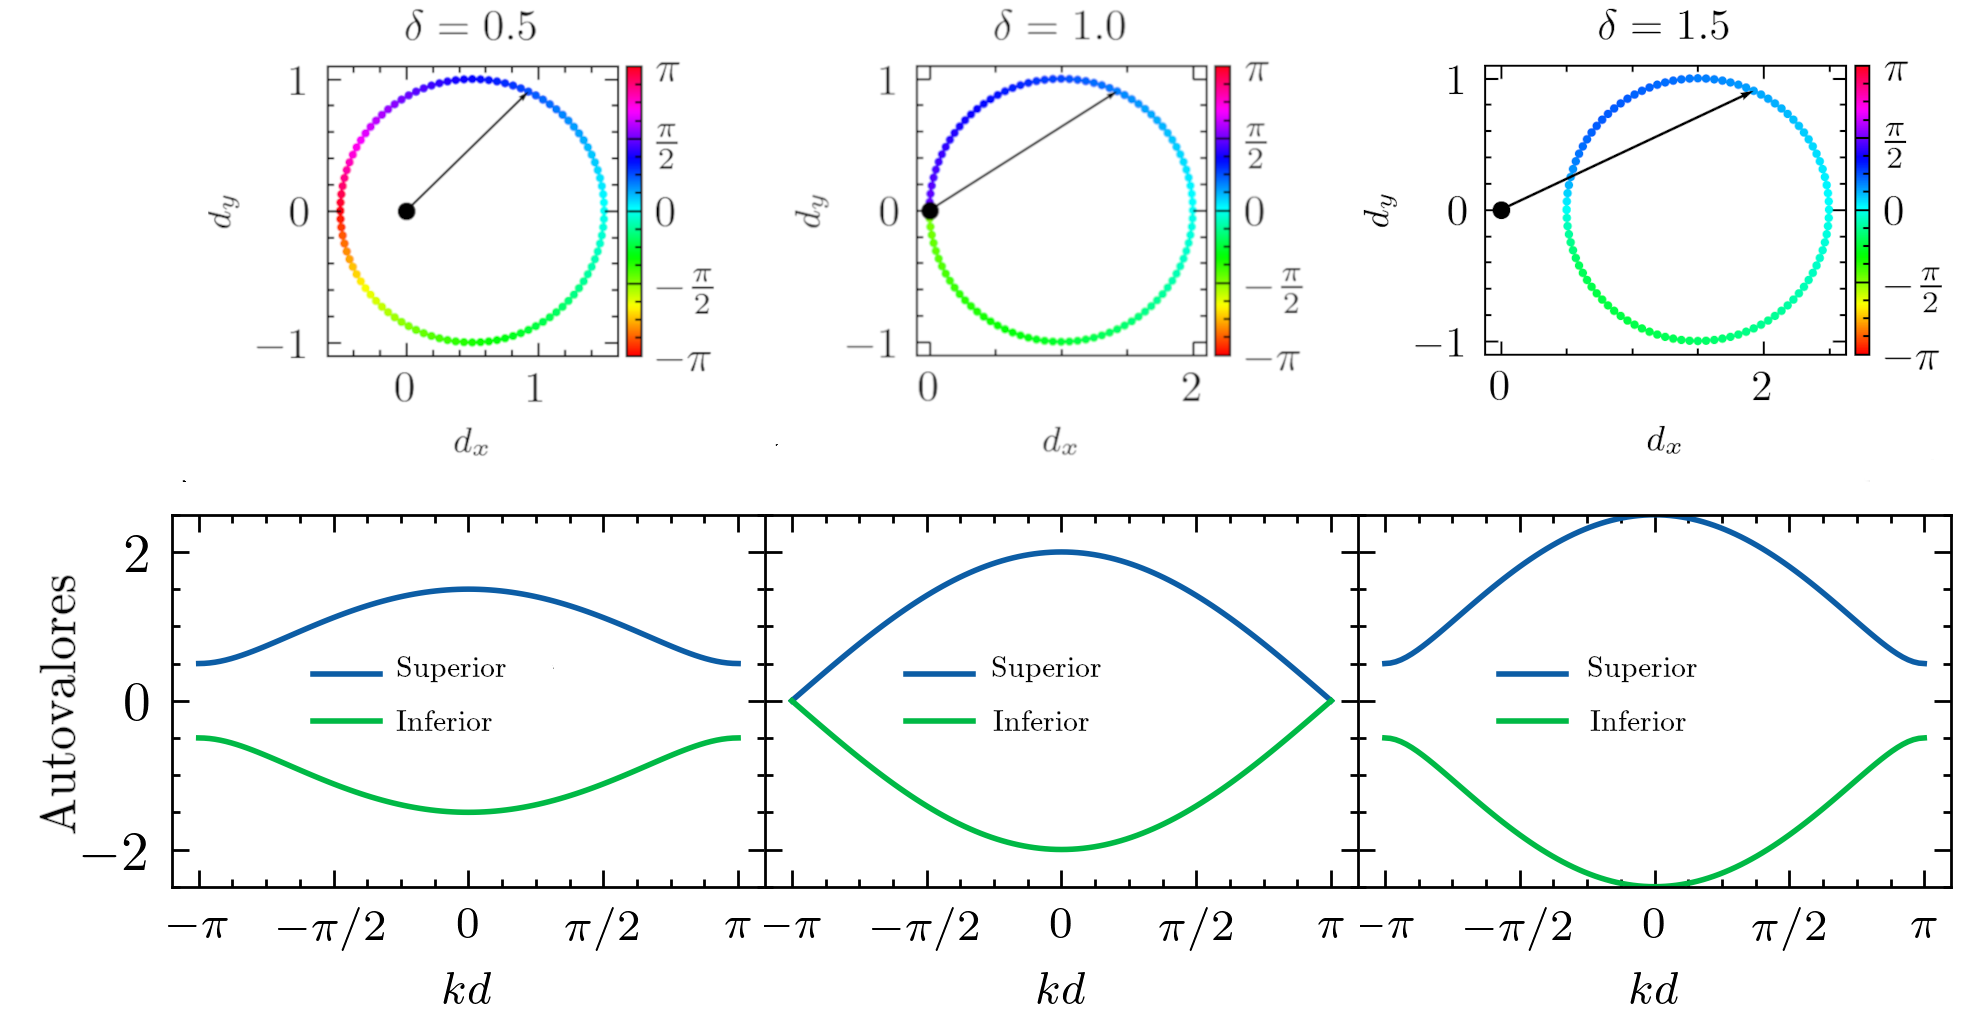
\includegraphics[width=\linewidth]{media/ssh-winding}
\caption[Topology of the SSH lattice.]{Topology of the SSH lattice. Top: Vectors $\textbf{d}$(k) and their phase. For $\delta < 1$ ($\delta > 1$), the origin is (not) enclosed. Bottom: Bands as a function of quasimomentum $k$ in the first Brillouin zone for $\delta < 1$, $\delta = 1$ and $\delta > 1$. Here $t'=1$ is fixed and $\delta'$ is varied for a number $N=100$  of unit cells.
	\label{fig:ssh-topo}}
\end{figure} \begin{figure}[h]
\centering	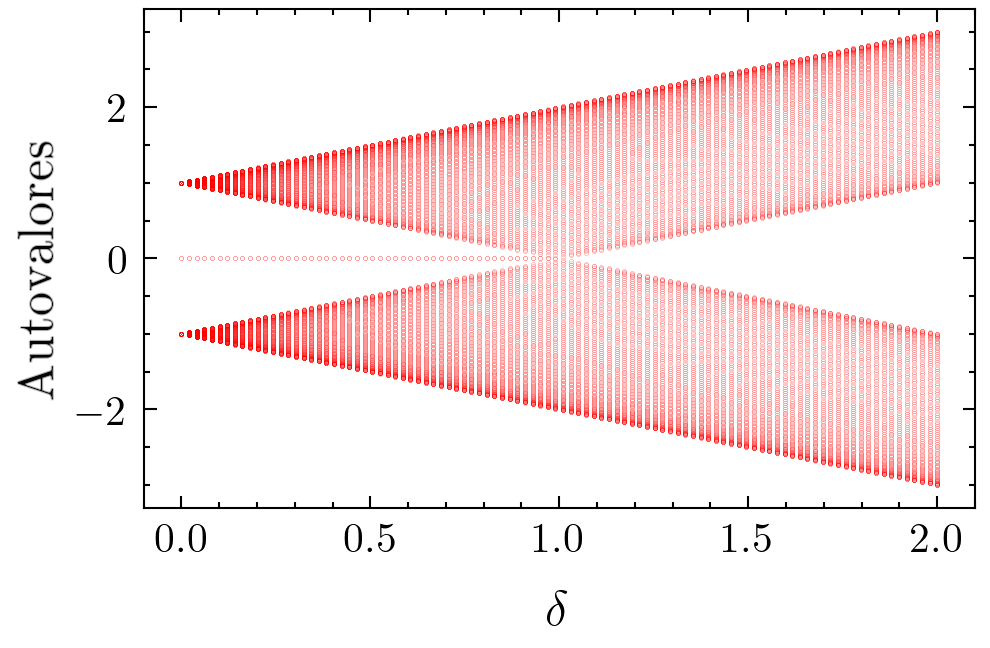
\includegraphics[width=0.7\linewidth]{media/ssh-open}
	\caption[Spectrum of the finite SSH lattice.]{Spectrum of the finite SSH lattice. The emergence of zero-energy edge states for $\delta < 1$ is observed. Open boundary conditions as a function of the parameter $\delta=t/t'$, with fixed $t'=1$  and a number $N=100$ of unit cells.
		\label{fig:ssh-open}}
\end{figure} 
